\chapter{Sparse Grids \textit{\&} Learning}

\section{Sparse Grids}
Sparse grids is a discretization technique that originates from numerical partial differential equations.
Even though they can be used for a diverse set of problems, we will only build up the exact amount of theory that is useful for our further study.

This chapter starts with a short description of the adaptive sparse grid technique and then progresses to our application of choice: supervised learning.
The discussion of sparse grids follows~\cite{bungartzSparse,spatAdaptGrid,sparse-parsimony}.

\subsection{Basis functions}
\sidetitle{1-Dimensional Basis}
As our first building stone we define the \enquote{mother hat} function
\begin{equation*}
  \label{eq:mother-hat}
  h(x) = \max \left( 1 - \vert x \vert , 0 \right).
\end{equation*}
We now define a one-dimensional linear basis function for a level \(l\) and an
odd index \(i \leq 2^{l} - 1\) by
\begin{equation}
  \label{eq:oned-basis}
  \varphi(x)_{l, i} = h(2^l x - i).
\end{equation}
The basis function defined by the former equation are called the linear basis functions~\cite{bungartzSparse}.
These basis functions assume that the function we want to approximate is zero on the boundaries.
This is why we use the similarly constructed ``modified linear basis functions'', as defined by Pflüger in~\cite{spatAdaptGrid}:
\newlength{\ldiff}
\setlength{\ldiff}{\widthof{$2^l x - i + 1$}-\widthof{$2 - 2^l x$}}
\begin{equation*}
\varphi_{l,i} (x) =
  \begin{cases}
    1 & \text {if } l = 1 \land i = 1,\\
    \begin{cases}
      2 - 2^l x & \hspace{\ldiff} \text{if } x \in [0, 2^{1-l}], \\
      0 & \hspace{\ldiff} \text{otherwise},
    \end{cases} & \text{if } l > 1 \land i = 1,\\
    \begin{cases}
      2^l x - i + 1 & \text{if } x \in [1 - 2^{1-l}, 1],\\
      0 & \text{otherwise},
    \end{cases} & \text {if } l > 1 \land i = 2^l - 1,\\
    h(2^l x - i) & \text{otherwise}.
  \end{cases}
\end{equation*}
They are identical to the linear basis functions~(\ref{eq:oned-basis}), except on the boundaries, where they use extrapolation.
Note that the modified linear basis is constant for level one.
A visualization of all one dimensional basis functions for level three can be
seen in \cref{fig:oned-basis}.
Note that they are placed on a regular one-dimensional grid.

\begin{figure}[H]
  \centering
  \begin{subfigure}[c]{0.4\textwidth}
  \centering
  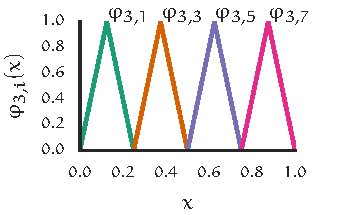
\includegraphics{lin_1d_3}  
  \caption{Linear basis}
  \end{subfigure}~
  \begin{subfigure}[c]{0.4\textwidth}
  \centering
  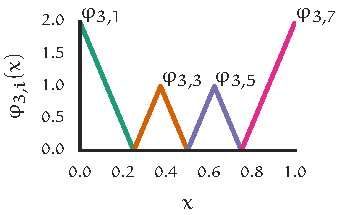
\includegraphics{lin_mod_1d_3}  
  \caption{Modified linear basis}
  \end{subfigure}
\caption{One dimensional basis functions for level three.}
  \label{fig:oned-basis}
\end{figure}

We define the useful shorthand notation of multi-indices, which represent a
collection of indices.
Arithmetical functions act on multi-indices element-wise, as does the relation
\begin{equation*}
  \bm{\alpha} \leq \bm{\beta} \iff \forall i\colon \alpha_i \leq \beta_i.
\end{equation*}
The \(l_1\) and the maximum-norm are defined for multi-indices by
\begin{equation*}
  \vert \bm{\alpha} \vert_1 = \sum_{\mathclap{1 \leq i \leq d}} \alpha_i, \,  \vert \bm{\alpha} \vert_\infty = \max_{1 \leq i \leq d} \alpha_i.
\end{equation*}
We use \(\bm{1}\) and \(\bm{2}\) as a short-hand for \((1, \ldots, 1)\) and
\((2, \ldots, 2)\) respectively.

\sidetitle{\(d\)-Dimensional Basis}
We can then construct the \(d\)-dimensional basis functions with the tensor product construction
\begin{equation*}
\varphi_{\bm{l}, \bm{i}} (\bm{x}) = \prod_{k=1}^d \varphi_{l_k, i_k} (x_k),
\end{equation*}
where \(\bm{l}\) corresponds to the levels and \(\bm{i}\) to the indices used by the basis function~\cite{bungartzSparse}.

\subsection{Full \textit{\&} Sparse Grids}
\begin{figure}[htb]
  \centering
  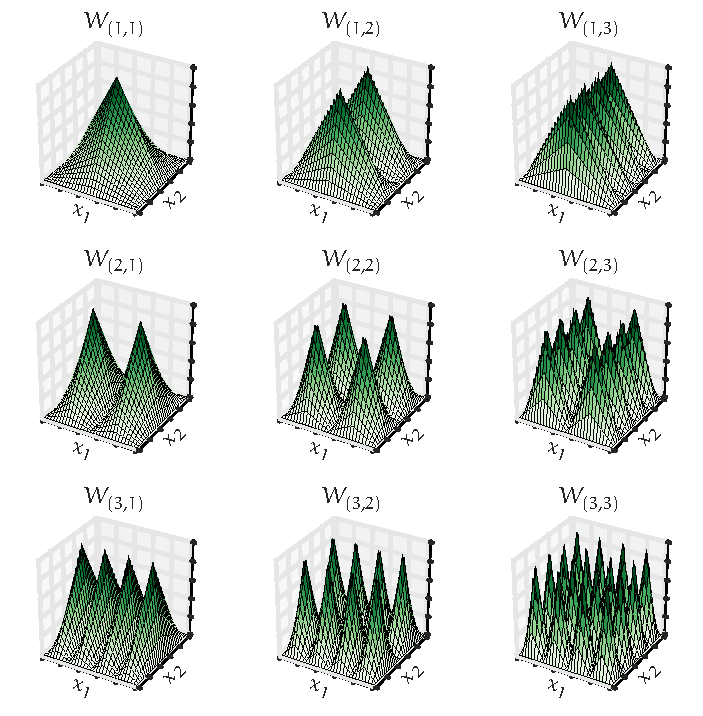
\includegraphics{lin_2d_3}
  \caption{Hierarchical two-dimensional subspaces up to level three.
  With standard linear basis functions.}\label{fig:hier-subspaces}
\end{figure}
\sidetitle{Hierarchical Subspaces}
Using the index-set~\cite{sparse-parsimony}
\begin{equation*}
 G_{\bm{l}} = \{(\bm{l, i}) \in \mathbb{N} \times \mathbb{N} \, \mid 1 \leq i_t \leq 2^{l_t} -1,\, i_t \text{ odd},\, 1 \leq t \leq d\},
\end{equation*}
the \(d\)-dimensional basis functions span the hierarchical subspaces
\begin{equation*}
  W_{\bm{l}} = \operatorname{span}\{\phi_{\bm{l},\bm{i}} \, \mid (\bm{l}, \bm{i}) \in G_{\bm{l}}\}.
\end{equation*}
\Cref{fig:hier-subspaces} shows all two-dimensional subspaces up to level three.
Note that the basis functions are placed on a regular grid.

\sidetitle{Full Grid}
Using those subspaces, we can create the set of grid points \(G_n^{-\infty}\) of the full grid for a level \(n\) and its corresponding approximation space \(V_n^{-\infty}\)
\begin{align*}
  G_n^{-\infty} &= \bigcup_{\mathclap{\vert {\bm{l}} \vert_\infty \leq n}} G_{\bm{l}}, \\
  V_n^{-\infty} &= \bigoplus_{\mathclap{\vert {\bm{l}} \vert_\infty \leq n}} W_{\bm{l}}.
\end{align*}
The number of basis functions of the full grid approximation space \(\vert V_n^{-\infty} \vert\) is in \( \BigO (2^{nd})\).
We can represent every function \(f(\bm{x})\) in \(V_n^{-\infty}\) by
\begin{equation}\label{eq:coefficients-h2mix}
  f(\bm{x}) = \sum_{g\, \in \bm{G_l}} \alpha_{g} \varphi_{g}(\bm{x}),
\end{equation}
as a sum over all grid points that is weighted by the so called hierarchical coefficients or surpluses \(\alpha_{g}\).

\sidetitle{Function Space}
Let \(\Omega = [0, 1]^d\) represent a \(d\)-dimensional interval. 
We now consider functions \({f \from \Omega \to \mathbb{R}}\) with bounded weak
mixed second derivatives
\begin{equation*}
  D^{\bm{k}} f = \frac{\partial^{\vert \bm{k} \vert_1 }}{\partial x^{k_1}_1 \cdots \partial x^{k_d}_d} f,
\end{equation*}
where \(\bm{k}\) is a \(d\)-dimensional multi-index.
In other words, we consider functions that are sufficiently smooth.
These functions form the Sobolev space~\cite{sparse-parsimony}
\begin{equation*}
  H_2^\text{mix}(\Omega) = \{ f \from \Omega \to \mathbb{R} \, \mid  D^{\bm{k}} f < \infty, \vert \bm{k} \vert_\infty \leq 2, f \rvert_{\partial \Omega = 0}\}.
\end{equation*}

\sidetitle{Sparse Grid}
For this function space sparse grids is a discretization method that represents a reasonable trade-off between accuracy and efficiency.
By exchanging the \(l_\infty\) with the \(l_1\)-norm we get
\begin{align}
  G_n^0 &= \bigcup_{\vert {\bm{l}} \vert_1 \leq n + d - 1} G_{\bm{l}}, \nonumber \\
  V_n^0 &= \bigoplus_{\vert {\bm{l}} \vert_1 \leq n + d - 1} W_{\bm{l}} \label{eq:sparse-grid-space},
\end{align}
which correspond to the grid point set and the approximation space of sparse
grids respectively~\cite{bungartzSparse}.
Again, we can split every function \(f(\bm{x}) \in V_n^0\) into a weighted sum
over all basis functions.
A sparse grid for a level \(n\) has only \(\vert G_n^0 \vert \in \BigO (2^n
n^{d-1})\) grid points.
\Cref{fig:full-vs-sparse} shows a visualization of both grid types for a
two-dimensional grid with level four.

\begin{figure}[H]
  \centering
  \begin{subfigure}[b]{0.23\textwidth}
    \centering
    \includegraphics[width=\textwidth]{{{grid_T-inf}}}
    \caption{Full Grid}
  \end{subfigure}
   \begin{subfigure}[b]{0.23\textwidth}
    \centering
    \includegraphics[width=\textwidth]{{{grid_T0}}}
    \caption{Sparse Grid}
  \end{subfigure}
  \caption{Grid visualization for 2-dimensional grids with level four.}\label{fig:full-vs-sparse}
\end{figure}

\subsection{Adaptivity}
Sparse grids work best if the function adheres to our smoothness assumptions.
Functions that are not well behaved, such as functions that are not smooth in
some parts of their domain, are more difficult to handle.
\citeauthor{spatAdaptGrid} devised an adaptive technique that helps us to approximate challenging functions in~\cite{spatAdaptGrid}.
Instead of relying only on the theoretically optimal results of sparse grids for
functions in \(H^2_{\text{mix}}\), he described an optimization process to
refine grids so that they adapt to the circumstances of the problem.

Because the ideal grid is computationally hard to calculate, a greedy algorithm that approximates the optimal solution is used~\cite{spatAdaptGrid}.
The idea is quite simple: we create new grid points that are likely to capture
additional information, close to existing points.
An example can be seen in \cref{fig:adaptivity}.
For a more elaborate discussion we refer the interested reader to~\cite{spatAdaptGrid}.

\begin{figure}[thb]
\centering
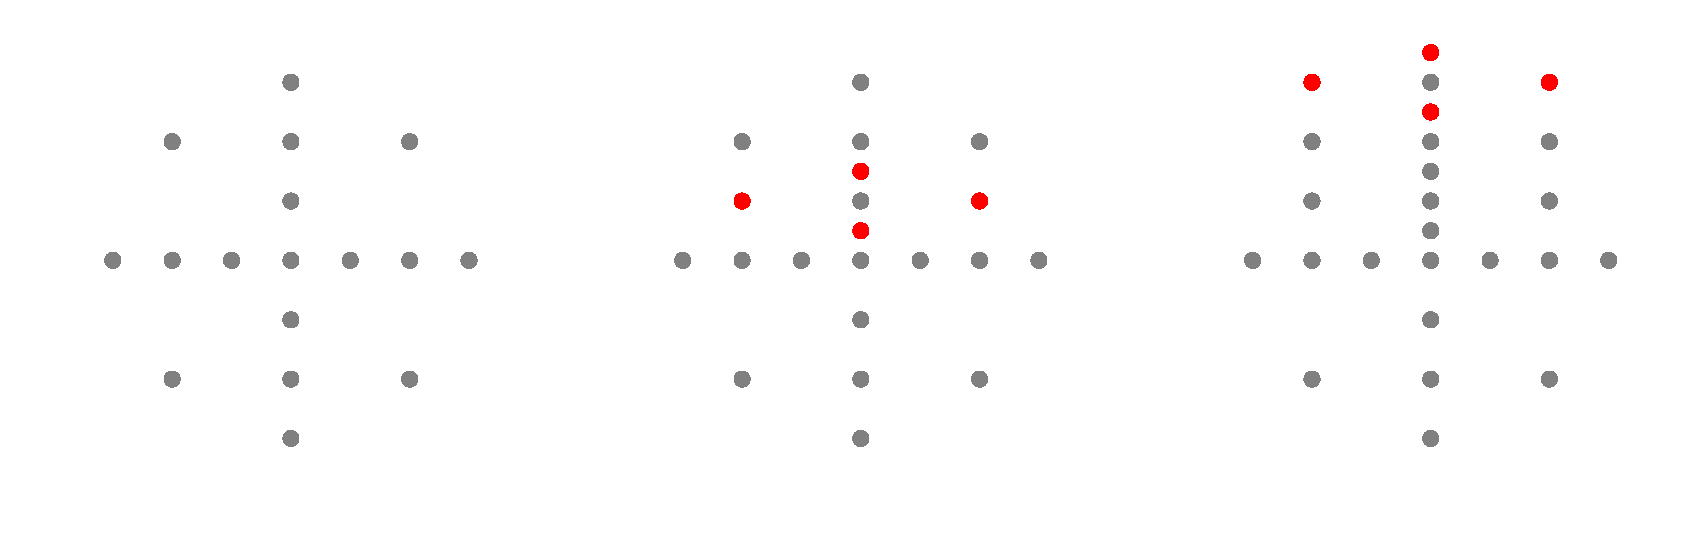
\includegraphics[width=1.0\textwidth]{adaptivity}
 \caption[Adaptivity]{We start with a small 2-dimensional grid with level 3. The first
   picture shows the standard grid, the other two show one adaptivity step each.
 The red points are the points created by the adaptivity step.}\label{fig:adaptivity}
\end{figure}

\section{Learning with Sparse Grids}
\sidetitle{Supervised Learning}
Let the set
\begin{equation*}
T = \left\{ \left(  \bm{x}_i, y_i \right) \right\}_i^n \subset [0,1]^d \times \bm{y}  
\end{equation*}
be a set of labelled examples with \(\bm{x} = x_1, x_2, \ldots, x_d\) as predictors and \(\bm{y}\) as the target variable. 
Predictors that are not in \([0,1]\) need to be scaled.
This set represents our dataset.
The goal is not interpolation, as we do not want to find a function that fits the examples exactly.
We rather want to find an approximation of our function that generalizes well,
i.e.~a function that captures the structure of the training data and can be
used to predict the target variable for different, yet unseen data points.

We differentiate between
\begin{description}
\item[Regression] if we want to predict a continuous \(y\),
\item[Classification] if we want to predict a discrete value, for example a class.
\end{description}
In this thesis we will mostly see examples of regression, the last chapter contains an example for a high-dimensional classification problem.

\sidetitle{Regression}
Let \(\bm{\phi}(\bm{x}) \from \mathbb{R}^d \to \mathbb{R}^{m \times 1}\) denote
a vector valued function consisting in all \(m\) \(d\)-dimensional basis
functions evaluated at a point \(\bm{x}\) with an associated weight vector \(\bm{\alpha} \in \mathbb{R}^{1 \times m}\).
We can then express our prediction for \(\bm{y}\) as
\begin{equation*}
\hat{\bm{y}}(\bm{x}) = \sum_{j = 1}^m \alpha_j \varphi_{j}(\bm{x}) = \boldsymbol{\alpha}^\intercal \bm{\phi} (\bm{x}),
\end{equation*}
which is a weighted sum of the basis functions, closely related to \cref{eq:coefficients-h2mix}.

\begin{figure}[htb]
  \centering
  \begin{subfigure}[b]{0.4\textwidth}
    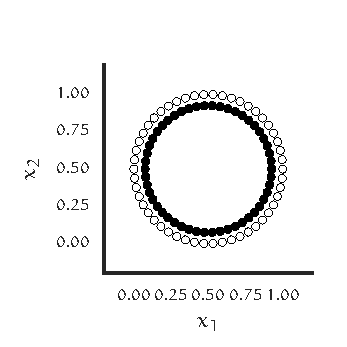
\includegraphics{circle}
    \caption{Original data.}
  \end{subfigure}
  \begin{subfigure}[b]{0.4\textwidth}
    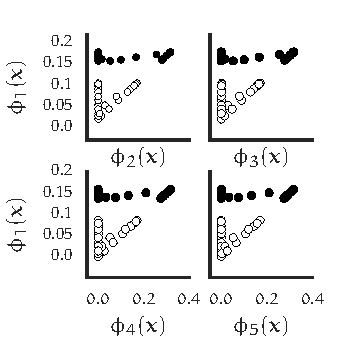
\includegraphics{feature_trans}
    \caption{Sparse grid perspective of the data.}
  \end{subfigure}
  \caption{Feature transformation for the circle dataset using a level two grid
    with standard linear basis.}
  \label{fig:features}
\end{figure}

\sidetitle{Feature Transformation}
We can view the sparse grid model as a feature map that transforms the originally
\(d\)-dimensional dataset into a new \(m\)-dimensional dataset, where one basis function represents one dimension of the sparse grid approximation space~\cite{sparse-parsimony}.
A simple example is shown in \cref{fig:features}.
We can see that the original dataset is not linearly separable, while the sparse
grid representation is.
Usually we have more dimensions \(m\) than original dimensions \(n\).
We then define the model matrix \(\bm{\Phi} \in \mathbb{R}^{n \times m}\) as
\begin{equation*}
\bm{\Phi}(\bm{x}) = \begin{bmatrix}
\phi_1(x_1) & \phi_2(x_1) & \hdots & \phi_m(x_1) \\
\phi_1(x_2) & \phi_2(x_2) & \hdots & \phi_m(x_2) \\
\vdots & \vdots & \ddots & \vdots \\
\phi_1(x_n) & \phi_2(x_n) & \hdots & \phi_m(x_n)
\end{bmatrix},
\end{equation*}
where each row corresponds to one datum of the dataset and each column is one of \(m\) new features.

\sidetitle{Optimization}
We can then perform linear regression using the matrix \(\bm{\Phi}\) as our
design matrix.
This perspective is useful, because it relates classical statistical methods with sparse grid learning and thus allows us to share common results.
The optimization goal is then given by
\begin{equation}\label{eq:optGoal}
\min_{\bm{\alpha}} \left\Vert  \bm{\Phi} \bm{\alpha} - \bm{y}   \right\Vert_2^2  + n \lambda \mathcal{S}(\bm{\alpha}), 
\end{equation}
where \(\mathcal{S}(\bm{\alpha})\) is a regularization operator and \(\lambda\) is a constant.
The regularization parameter \(\lambda\) is scaled by the number of data points \(n\).
This least-square problem can be solved for differentiable \(\mathcal{S}\) by a gradient-based solver.

Adaptivity can be integrated into this process by performing a refinement step after solving the optimization step, iterating until a satisfactory performance is achieved.
We select the points that should be refined by calculating the mean squared error (\textsc{mse}) for the model and then refine the grid, starting with the points with the highest contribution to the error.

\sidetitle{Classification}
A binary classification problem can be transformed into a regression problem by relaxing the target \(\bm{y}\).
We set \(y_i = 0\) for each data point when the datum belongs to the first class and \(y_i = 1\) if it does not.
The prediction of the model can then be interpreted as a certainty that the datum is a member of the class.

To solve a multi-class-classification problem, one-vs-all classification is used, for which we transform the problem into multiple binary classification problems.
We predict the target for an unseen data point by calculating the results for
each binary estimator and then report the class label of the learner that returned the largest certainty.

This implies that all methods that improve the performance of the regression procedure also very likely lead to better classification results because we are performing classification via regression.

\section{Software}
Throughout this thesis we will use the following libraries:
\begin{description}
\item[SG++] is a sparse grid toolbox implemented in \emph{C++}. This library was used for all
  experiments and contains all needed methods to recreate our experiments.
  Every method described in the following chapters was integrated into
  \emph{SG++}~\cite{spatAdaptGrid}.
\item[Scikit-Learn] is a Python machine learning library.
  We used it to implement cross-validation procedures and to perform
  grid-searches for hyper-parameter tuning~\cite{software-sklearn}.
\item[BayesOpt] is an implementation of Bayesian optimization procedures.
  It was used for hyper-parameter search as well~\cite{software-bayesOpt}.
\item[Matplotlib] is a popular Python plotting library with which we created all
  graphics~\cite{software-matplotlib}.
\end{description}

%%% Local Variables:
%%% mode: latex
%%% TeX-master: "../main"
%%% End: